\addbibresource{reference.bib}

\chapter{Atlas TPX}\label{atlas}
\todo popis AtlasTPX

\section{Atlas MPX}\label{atlas:mpx}
Atlas MPX\cite{Vykydal200935}\cite{atlasmpx} je předchůdcem detektorové sítě Atlas TPX, kterou v současné době je plně nahrazena. Skládala se z 16 Medipix2 detektorů, které byly instalovány na různé pozice Atlas detektoru - viz obr. \ref{fig:mpx_positions}. Hlavním cílem této sítě bylo měření vlastností radiačního pole atlasu, jeho složení, spektroskopických charakteristik a částečně také přispěla k měření neutronů. 

\begin{figure}[ht]
	\begin{center}
		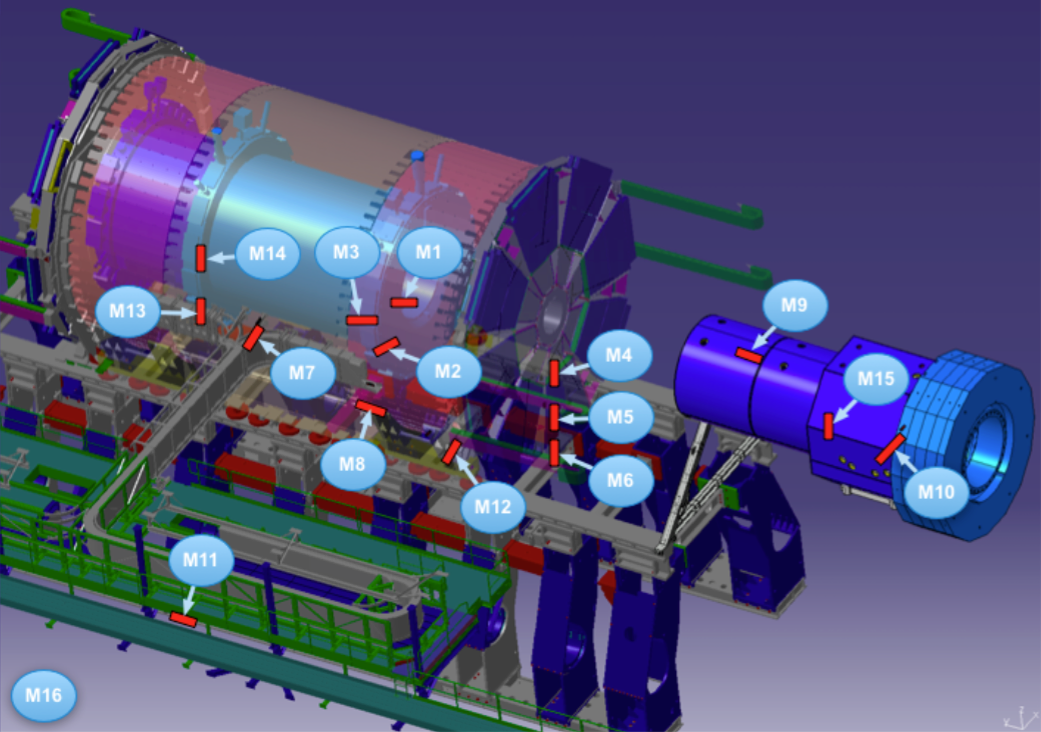
\includegraphics[width=11cm]{figures/mpx_positions.png}
		\caption{Atlas MPX s přehledem rozmístění detektorů}
		\label{fig:mpx_positions}
	\end{center}
\end{figure}

Všechny detektory operovaly v tzv. \texttt{Medipix módu}, který se vyznačují tím, že v rámci jedné akvizice počítá počet částic, které interagovaly pixelovou maticí detektoru a jejichž deponovaná energie byla vyšší, než prahová. Na obrázku \ref{fig:mpx_cluster} je znázorněn snímek z jednoho detektoru s detailem zachycených částic. Na obrázku vpravo nahoře je částice typu \texttt{heavy blob} (těžce nabitá částice, jejíž trajektorie byla kolmá s povrchem detektoru), vpravo dole je pak zachycena částice typu \texttt{heavy track} (také těžce nabitá částice, která ale přiletěla pod větším a proto zanechala větší stopu) - více klasifikaci částic se dočtete v podkapitole \ref{det:ca}.



\begin{figure}[ht]
	\begin{center}
		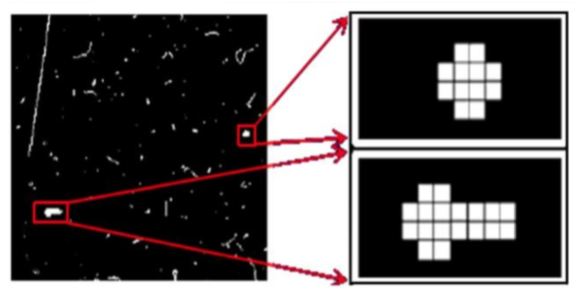
\includegraphics[width=7cm]{figures/mpx_cluster.png}
		\caption{Snímek z Atlas MPX detektoru s výřezem zachycených částic (převzato z \cite{atlasmpx})}
		\label{fig:mpx_cluster}
	\end{center}
\end{figure}


Každý z těchto detektorů byl osazen $300~\mu m$ tlustým křemíkovým senzorem, který byl pokryt konvertory pro lepší detekční účinnost neutronů (obr. \ref{fig:mpx_lay}).

\begin{figure}[ht]
	\begin{center}
		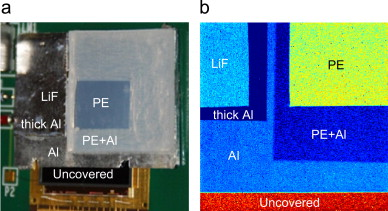
\includegraphics[width=7cm]{figures/mpx-layers.jpg}
		\caption{Fotografie znázorňující Medipix2 detektor s neutronovými konvertory (převzato z \cite{Vykydal200935})}
		\label{fig:mpx_lay}
	\end{center}
\end{figure}

\subsection{Hardwarová a softwarová architektura}
Tato síť se skládala z 16 \texttt{Medipix2} \ref{det:med} detektorů, které byly pomocí USB vyčítacího rozhraní \texttt{FITPix} \ref{det:fitpix} připojeny ke třem počítačům (z důvodu distribuce toku dat a výkonu). Na každém počítači se o komunikaci s detektory staral software \texttt{Pixelman} \ref{det:pixelman}, který řídil akvizici dat, nastavování parametrů detektorů apod. 

Pro vzdálené obládání každého byl vyvinut plugin pro Pixelman, který umožňoval jeho rozšíření o TCP/IP ovládací vrstvu. Pomocí jednoduchého textového protokolu bylo tedy možné řídit každý ze třech uzlů. Pro tyto účely byla vyvinuta centrální řídící aplikace \cite{Turecek2011S45}, pomocí které bylo možné řídit řídit akvizici všech detektorů a nastavovat jejich parametry. Tato aplikace poskytovala webové rozhraní (obr. \ref{fig:mpx_web}), které díky tou dobou méně striktní CERNské politiky síťové bezpečnosti bylo možné tento experiment ovládat z internetu.

\begin{figure}[ht]
	\begin{center}
		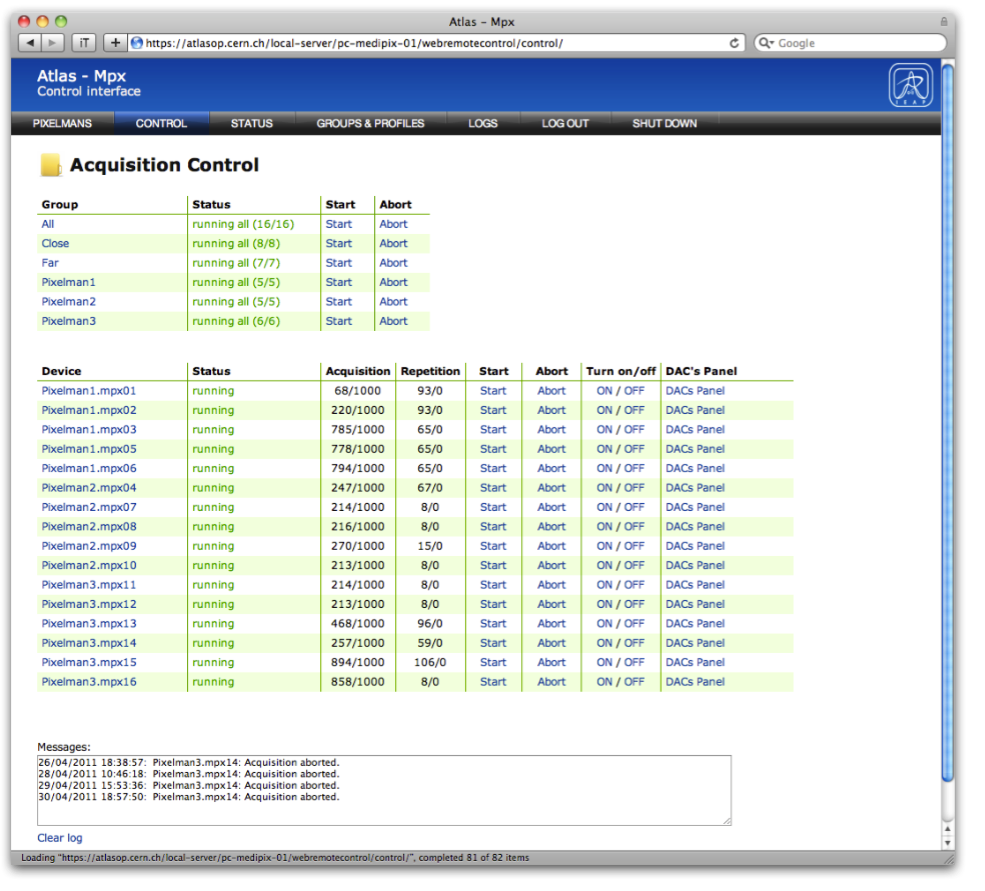
\includegraphics[width=10cm]{figures/mpx_web.png}
		\caption{Atlas MPX - řídící aplikace (převzato z \cite{TurecekThesis2011})}
		\label{fig:mpx_web}
	\end{center}
\end{figure}



